
% Template for ICASSP-2013 paper; to be used with:
%          spconf.sty  - ICASSP/ICIP LaTeX style file, and
%          IEEEbib.bst - IEEE bibliography style file.
% --------------------------------------------------------------------------
\documentclass{article}
\usepackage{spconf,amsmath,graphicx}
\usepackage{tikz}
\usetikzlibrary{positioning}
\tikzset{font=\footnotesize,>=stealth}
%\usepackage{dblfloatfix}
\usepackage{amsmath}
\usepackage{graphicx}
\usepackage{caption}
\usepackage{subcaption}
\usetikzlibrary{shapes,snakes}
\usetikzlibrary{calc,chains}
\usepackage{graphics,color}
\usetikzlibrary{plotmarks}
\usepackage{url}
\usepackage{pgfplots}
\usepackage[bottom]{footmisc}
\usetikzlibrary{plotmarks}
% Example definitions.
% --------------------
\def\x{{\mathbf x}}
\def\L{{\cal L}}
\def\ninept{\def\baselinestretch{.906}\let\normalsize\small\normalsize}

% Title.
% ------
\title{Frequency-Domain Single-Channel Inverse Filtering \\ for Speech Dereverberation: Theory and Practice}
%
% Single address.
% ---------------
\name{Ina Kodrasi, Timo Gerkmann, Simon Doclo
\thanks{
This work was supported in part by a Grant from the GIF, the German-Israeli Foundation for Scientific
Research and Development, the Cluster of Excellence 1077 ``Hearing4All'', funded by the German Research Foundation (DFG), and the Marie Curie Initial Training Network DREAMS (Grant no. 316969).
}}
\address{
University of Oldenburg, Department of Medical Physics and Acoustics, Oldenburg, Germany
}
\begin{document}
\newlength\figureheight
\newlength\figurewidth
\setlength\figureheight{5cm}
\setlength\figurewidth{6.2cm}
\ninept
%
\maketitle
%
\begin{abstract}
The objective of single-channel inverse filtering is to design an inverse filter that achieves dereverberation while being robust to an inaccurate room impulse response~(RIR) measurement or estimate.
Since a stable and causal inverse filter typically does not exist, approximate time-domain inverse filtering techniques such as single-channel least-squares~(SCLS) have been proposed. 
However, besides being computationally expensive and often infeasible, SCLS generally leads to distortions in the output signal in the presence of RIR inaccuracies.

In this paper, a theoretical analysis is initially provided, showing that the direct inversion of the acoustic transfer function in the frequency-domain generally yields instability and acausality issues.
In order to resolve these issues, a novel frequency-domain inverse filtering technique is proposed that incorporates regularization and uses a single-channel speech enhancement scheme. 
Experimental results demonstrate that the proposed technique yields a higher dereverberation performance and has a significantly lower computational complexity compared to the SCLS technique.



\end{abstract}
%
\begin{keywords}
acoustic single-channel inversion, stability, causality
\end{keywords}
%

\section{Introduction}
Speech dereverberation techniques are crucial for improving speech intelligibility, perceptual speech quality, and the performance of automatic speech recognition systems in reverberant environments~\cite{Jeub_ITASP_2010,Maas_ICASSP_2012}.
When the room impulse response~(RIR) between the source and the microphone can be measured or estimated, an inverse filter can be designed to invert the RIR, and hence, achieve dereverberation~\cite{Neely_1979,Mourjopoulos_1982,Jan_ICASSP_96}.
Although such an approach sounds attractive in theory, designing and applying an inverse filter results in several drawbacks in practice. 
Acoustic transfer functions are generally mixed-phase functions~\cite{Neely_1979} and therefore a stable and causal inverse filter does not exist.
Furthermore, the inverse filter is typically designed using an inaccurate RIR, where inaccuracies can arise from temperature variations~\cite{Hikichi_EURASIP_2007}, spatial mismatch~\cite{Radlovic_ITSA_2000}, or the sensitivity of blind system identification methods to near-common zeros and interfering noise~\cite{Hasan_EUSIPCO_2006}.
This will commonly lead to distortions in the output signal~\cite{Radlovic_ITSA_2000}.

In order to overcome some of these issues, alternative techniques such as single-channel least-squares~(SCLS)~\cite{Mourjopoulos_1982} and homomorphic inverse filtering~\cite{Mourjopoulos_1982,Radlovic_2000} have been investigated. 
In SCLS, the squared error between the output of the system and a desired response is minimized. 
In homomorphic inverse filtering, the RIR is first decomposed into a minimum-phase component and a maximum-phase component. An exact time-domain inverse filter is designed for the minimum-phase component, whereas the maximum-phase component is only approximately inverted using a delay and truncation. 
In a comparative study between SCLS and homomorphic inverse filtering in~\cite{Mourjopoulos_1982}, it has been concluded that SCLS yields a superior dereverberation performance. 
However, the SCLS inverse filtering technique still results in several drawbacks in practice. 
The RIR can be several thousand taps long, resulting in a computationally complex and often infeasible inverse filter design~\cite{Naylor_IWAENC_2005}. 
Furthermore, the output signal is often distorted when the SCLS filter is designed using an inaccurate RIR~\cite{Naylor_IWAENC_2005}.

In this paper, first a theoretical analysis is provided, showing that the direct inversion of the acoustic transfer function in the frequency-domain typically yields instability and acausality issues, giving rise to undesirable tones and pre-echoes.
A frequency-domain inverse filtering technique is then proposed, which incorporates regularization to reduce the tones and uses a single-channel speech enhancement scheme to reduce the pre-echoes. 

\section{Problem Formulation}
\label{sec: prob}
Consider a single-channel acoustic system, where the reverberant microphone signal $x(n)$ at time index $n$ arises from the convolution of the clean speech signal $s(n)$ with the time-invariant RIR $h(n)$ of length $L_h$, i.e., 
\begin{equation}
\label{eq: conv}
x(n) = s(n)\ast h(n).
\end{equation}
In order to recover the clean speech signal, an inverse filter $g(n)$ should be designed such that
\begin{equation}
\label{eq: gtime}
h(n) \ast g(n) = d(n),
\end{equation}
with
\begin{equation}
  \left\{
  \begin{array}{lcl}
    d(n) & = & 1 \; \; {\text{at}} \; \; n = 0,\\
    d(n) & = & 0 \; \; {\text{elsewhere}}.
  \end{array}
  \right.
\end{equation}
In~\cite{Neely_1979} it has been experimentally validated that acoustic transfer functions are typically mixed-phase functions, such that a causal and stable inverse filter does not exist.
Alternatively, the SCLS technique~\cite{Mourjopoulos_1982} has been proposed, which aims at designing an approximate inverse filter.
In SCLS, a time-domain filter $\mathbf{g}$ of length $L_g$ is designed, with $\mathbf{g} = [g(0) \; g(1) \; \ldots \; g(L_g-1)]^T$, by expressing~(\ref{eq: gtime}) in terms of a matrix/vector multiplication as 
\begin{equation}
\mathbf{H}\mathbf{g} = \mathbf{d},
\end{equation}
with $\mathbf{H}$ being the $(L_h + L_g -1) \times L_g$-dimensional convolution matrix of $h(n)$ and $\mathbf{d}$ being the $(L_h+L_g-1) \times 1$-dimensional desired response vector $\mathbf{d}  = [1 \; 0 \; \ldots \; 0]^T$.
Minimizing the least-squares error $J_{\rm SCLS} = \|\mathbf{H}\mathbf{g} - \mathbf{d} \|_2^2$ yields the SCLS filter 
\begin{equation}
\label{eq: ls}
\mathbf{g}_{\rm _{SCLS}} = (\mathbf{H}^T\mathbf{H})^{-1}\mathbf{H}^T\mathbf{d}.
\end{equation}
Designing and using $\mathbf{g}_{\rm _{SCLS}}$ however encounters several drawbacks in practice. 
The true RIR is generally not available and should either be measured beforehand or estimated~\cite{Huang_ITSP_2003}.
Independently of whether the RIR is measured or estimated, there is typically a mismatch between the true RIR $h(n)$ and the available RIR $\hat{h}(n)$~\cite{Hikichi_EURASIP_2007,Radlovic_ITSA_2000,Hasan_EUSIPCO_2006}.
The SCLS filter designed using the inaccurate $\hat{h}(n)$ may fail to achieve dereverberation, leading to distortions in the output signal~\cite{Naylor_IWAENC_2005}.
Furthermore, $\hat{h}(n)$ can be several thousand taps long, resulting in a computationally complex, numerically unstable, and often infeasible filter design~\cite{Naylor_IWAENC_2005}, due to the multiplication and inversion of the high-dimensional convolution matrix in~(\ref{eq: ls}). 

In order to avoid the inversion of the convolution matrix, a frequency-domain inverse filter can be designed instead.
Consider the STFT-representation of the signal model in~(\ref{eq: conv}), i.e.,
\begin{equation}
  \label{eq: stft}
  X(k,l)= S(k,l) H(k),
\end{equation}
with $k = 0, \; \ldots, \; K-1,$ denoting the frequency index and $l$ denoting the frame index.
We assume that $K \geq L_h$, such that the convolution in~(\ref{eq: conv}) can be accurately represented by multiplication in the STFT-domain.
Given an estimate $\hat{H}(k)$ of the acoustic transfer function $H(k)$, an inverse filter $G(k)$ can be directly designed as
\begin{equation}
\label{eq: fi}
  G(k) = \frac{1}{\hat{H}(k)}.
\end{equation}
In this paper, we will first analyze the instability and acausality issues associated with $G(k)$ and show that applying this inverse filter will typically give rise to undesirable tones and pre-echoes.
A fast frequency-domain inverse filtering technique is then proposed, which aims at realizing a stable approximate inverse filter to avoid the tones as well as at reducing the pre-echoes arising due to acausality.

\section{Frequency-Domain Channel Inversion}
\subsection{Instability and acausality of $G(k)$}
\label{sec: analysis_z}
In this section, the fundamental concepts of analyzing the stability and causality of discrete-time systems via the $\cal{Z}$-transform and the region of convergence~(ROC) are briefly reviewed and used to show that using the frequency-domain inverse filter $G(k)$ in~(\ref{eq: fi}) encounters two main drawbacks: (i) the zeros of the RIR on the unit circle yield an unstable inverse filter, causing undesirable tones in the processed signal, and (ii)  the zeros of the RIR outside of the unit circle result in an acausal inverse filter, and thus in pre-echoes in the processed signal. 

The $\cal{Z}$-transform of a sequence $p(n)$ is defined as
\begin{equation}
  \label{eq: ztr}
  P(z) = \sum_{n = -\infty}^{\infty}p(n)z^{-n}, 
\end{equation}
while the ROC is defined as the set of complex numbers $z$ for which $P(z)$ converges.
For a filter to be stable, the ROC must include the unit circle, i.e., $|z| = 1$, whereas for a filter to be causal, the ROC must extend outward from the outermost pole.  
It should be noted that the $\cal{Z}$-transform is unique if and only if its ROC is also specified.
If a $\cal{Z}$-transform without a ROC is provided, an inverse $\cal{Z}$-transform can be determined based on whether stability or causality is desired~\cite{oppenheim_1996}.

Since $G(k)$ in~(\ref{eq: fi}) is related to the $\cal{Z}$-transform $G(z)$ of the inverse filter $g(n)$ by
\begin{equation}
\label{eq: fz}
G(k) = G(z) \Big |_{z = e^{j\frac{2 \pi k}{K}}},
\end{equation}
analysis of the ROC of $G(z)$ can be used to determine whether $G(k)$ realizes a stable or a causal filter. 

Fig.~\ref{fig: poleh}(a) depicts the pole-zero representation of a measured RIR from the MARDY database~\cite{Wen_IWAENC_2006}, with a zoomed in portion presented in Fig.~\ref{fig: poleh}(b).
\begin{figure}[b!]
  
  \hspace{0.6cm} 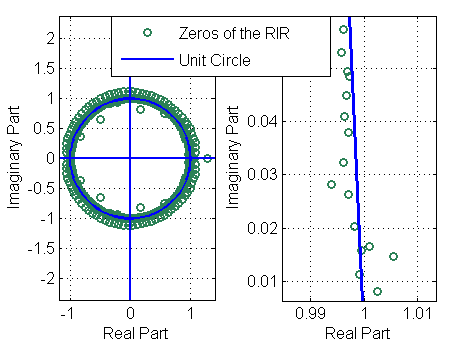
\includegraphics[scale=0.65]{plots/bode_plot}

  \hspace{2.7cm} (a) \hspace{3.4cm} (b)

  \caption{Pole-zero representation of a typical RIR.}
  \label{fig: poleh}
\end{figure}
As illustrated in this figure, the zeros of a typical RIR tend to cluster near the unit circle~\cite{Hughes_2008}, lying slightly inside, outside, and on the unit circle.
Hence, the inverse $G(z)$ of a typical RIR will contain poles inside, outside, and on the unit circle.
Given the relation in~(\ref{eq: fz}), clearly the poles of $G(z)$ on the unit circle will result in an unstable inverse filter $G(k)$, causing undesirable tones in the processed signal.
In the following, a simple illustrative example is presented demonstrating how the remaining poles of $G(z)$ inside and outside the unit circle affect the causality of the inverse filter $G(k)$ in~(\ref{eq: fi}).

{\it{Example 1: Consider the impulse response with transfer function $\hat{H}(z) = (1-0.5z^{-1})(1-2z^{-1})$. 
The $\cal{Z}$-transform of its inverse is given by
\begin{equation}
\label{eq: g1}
G(z) = \frac{1}{(1-0.5z^{-1})(1-2z^{-1})},
\end{equation}
with the pole at $z = 0.5$ and at $z = 2$ being inside and outside the unit circle, respectively.
The ROC of rational $\cal{Z}$-transforms has to be bounded by poles or extend to infinity~\cite{oppenheim_1996}, hence, for the rational $G(z)$ in~(\ref{eq: g1}) only $3$ different ROC definitions are possible, i.e., $|z|< 0.5$, $|z|> 2$, or $0.5<|z|< 2$.
When a frequency-domain inverse filter is designed as in~(\ref{eq: fi}), a finite response is obtained since $G(z) \neq \infty$ for $z = e^{j\frac{2 \pi k}{K}}$.
Therefore it can be said that $G(k)$ in~(\ref{eq: fi}) realizes the filter with the $\cal{Z}$-transform in~(\ref{eq: g1}) and the ROC including the unit circle, i.e., $0.5 < |z| < 2$.
The inverse $\cal{Z}$-transform of~(\ref{eq: g1}) with the ROC being $0.5 < |z| < 2$ is given by~\cite{oppenheim_1996}
\begin{equation}
\label{eq: iz}
g(n) = -\frac{1}{3} 0.5^n u(n) - \frac{4}{3} 2^n u(-n-1),
\end{equation}
with $u(n)$ denoting the unit step function. 
The sequence in~(\ref{eq: iz}) represents a stable bilateral filter, with a causal component due to the pole inside the unit circle and an acausal component due to the pole outside of the unit circle.}}

Based on this example, it can be concluded that for a typical RIR with zeros outside the unit circle, the inverse filter $G(k)$ in~(\ref{eq: fi}) results in acausal filtering of the microphone signal, hence yielding undesirable pre-echoes.

\begin{figure}[b!]
  \centering
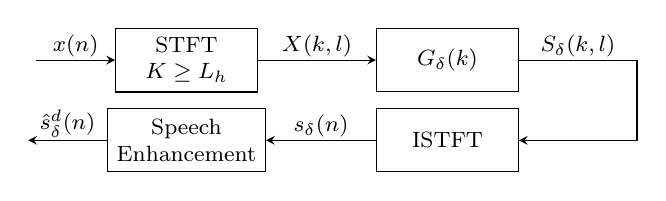
\begin{tikzpicture}
    \begin{scope}[every node/.style={align=center,draw,minimum width=1.8cm,minimum height=.8cm}]
      \node                      (stft)   {STFT \\ $K\ge L_h$};
      \node[right=1.5cm of stft] (g)      {$G_\delta(k)$};
      \node[below=.2cm of stft]  (speech) {Speech \\ Enhancement};
      \node at (g |- speech)     (istft)  {ISTFT};
    \end{scope}

    \begin{scope}[every node/.style={midway,above,inner sep=1pt}]
      \draw[<-] (stft.west) -- node {$x(n)$} ++(left:1cm);
      \draw[->] (stft.east) -- node {$X(k,l)$} (g.west);
      \draw[->] (g.east) -- node {$S_\delta(k,l)$} ++(right:1.5cm) |- (istft.east);
      \draw[->] (istft.west) -- node {$s_\delta(n)$} (speech.east);
      \draw[->] (speech.west) -- node {$\hat s^d_\delta(n)$} ++(left:1cm);
    \end{scope}
  \end{tikzpicture}
  \caption{Schematic representation of the proposed technique.}
  \label{fig: al_sche}
\end{figure}
\subsection{Frequency-Domain Single-Channel Dereverberation}
In order to overcome the previously described issues of instability and acausality, the frequency-domain inverse filtering technique depicted in Fig.~\ref{fig: al_sche} is proposed, where the undesirable tones and pre-echoes are reduced by incorporating regularization and a speech enhancement scheme.

\subsubsection{Designing a stable approximate inverse filter}

The advantage of a frequency-domain inverse filter design lies in the fact that the transfer function is being evaluated on the unit circle, hence the unstable poles can be directly manipulated.
In order to obtain a stable approximate inverse filter, we propose designing a regularized filter $G_{\delta}(k)$, i.e.,
\begin{equation}
  \label{eq: rfi}
  G_{\delta}(k) = \frac{\hat{H}^{*}(k)}{|\hat{H}(k)|^2 + \delta},
\end{equation}
where $\hat{H}^{*}(k)$ denotes the conjugate of $\hat{H}(k)$ and $\delta$ is a frequency-independent regularization parameter.
The incorporation of regularization moves the unstable poles of $G(z)$ on the unit circle inside the unit circle, hence replacing the unstable filtering components by causal filtering components~(c.f. Example $1$).
While regularization strongly reduces the tones in the processed microphone signal, the synthesized signal $s_{\delta}(n)$ exhibits pre-echoes due to the remaining acausality in $G_{\delta}(k)$.
To remove the acausality in $G_{\delta}(k)$, clearly the same approach as in homomorphic inverse filtering can be applied, i.e., delaying and truncating the inverse discrete Fourier transform of $G_{\delta}(k)$.
However, such an approach penalizes the achievable dereverberation performance and has been shown to be inferior to the SCLS technique. 

\subsubsection{Reducing the pre-echoes in the processed signal}
\label{sec: enh}
In order to reduce the pre-echoes in $s_{\delta}(n)$, we propose to apply a single-channel speech enhancement scheme which estimates the pre-echo power spectral density~(PSD) and employs this estimate to compute an enhancement gain function.
In the STFT-domain, $s_{\delta}(n)$ can be written as  
\begin{equation}
S_{\delta}(k',l') = S_{\delta}^d(k',l') + E(k',l'), 
\end{equation}
where $S_{\delta}^d(k',l')$ represents the desired speech spectral coefficients, $E(k',l')$ represents the spectral coefficients of the pre-echoes, $k' = 0, \; \ldots, \; K'-1,$ denotes the frequency index, and $l'$ denotes the frame index.
It should be noted that to account for the short-time stationarity of speech, the number of frequency bins $K'$ in this stage is $K' \ll K$.
Similarly to the commonly made assumption in spectral subtraction-based dereverberation techniques that the direct signal and late reflections are uncorrelated~\cite{Kinoshita_ITASLP_2009}, the direct desired speech $S_{\delta}^d(k',l')$ and the pre-echoes spectral coefficients $E(k',l')$ can be assumed to be uncorrelated in each observation frame.
Furthermore, given that the pre-echoes in $s_{\delta}(n)$ can be regarded as fairly non-stationary noise, we propose to estimate the PSD $\hat{\sigma}_E^2(k',l') = {\cal{E}} \{ |E(k',l')|^2 \}$ by employing the noise PSD estimator based on the speech presence probability with fixed priors~\cite{Gerkmann_2012}, since it has been experimentally validated that this estimator exhibits a fast tracking performance for non-stationary noise.
It should be noted that due to $K' \ll K$, $E(k',l')$ is significantly more stationary than $S_{\delta}^d(k',l')$, making it plausible for the noise PSD estimator in~\cite{Gerkmann_2012} to discriminate between desired speech and pre-echoes.

Using $\hat{\sigma}_E^2(k',l')$, the a priori SNR $\hat{\xi}(k',l')$ is then estimated using the cepstral smoothing approach proposed in~\cite{Breithaupt_2008}, with
\begin{equation}
\hat{\xi}(k',l') = \frac{{\cal{E}} \{ |S_{\delta}^d(k',l') |^2 \} }{\hat{\sigma}_{E}^2(k',l')}.
\end{equation}
Finally, a Wiener gain function $G_{\rm W}(k',l')$ is computed and applied to $S_{\delta}(k',l')$ to obtain an estimate of the desired speech spectral coefficients $\hat{S}_{\delta}^{\rm d}(k',l')$, i.e., $\hat{S}_{\delta}^{\rm d}(k',l') = G_{\rm W}(k',l')S_{\delta}(k',l')$, with
\begin{equation}
  G_{\rm W}(k',l') = \frac{\hat{\xi}(k',l')}{1+\hat{\xi}(k',l')}.
\end{equation}

\section{Experimental Results}
\label{sec: exp}
To investigate the performance of the proposed technique and compare it to the performance of SCLS, we have considered a measured RIR $\mathbf{h} = [h(0) \; \ldots \; h(L_h-1)]^T$ with reverberation time $T_{60} \approx 450$~ms as the true RIR to be inverted.
The sampling frequency is $f_s = 16$~kHz and the RIR length is $L_h = 7200$. 
The inaccurate RIR $\hat{\mathbf{h}} = [\hat{h}(0) \; \ldots \; \hat{h}(L_h-1)]^T$ used for the inverse filter design is simulated as in~\cite{Cho_ITSA_1999}, i.e., $\hat{h}(n) = h(n) \left[1+e(n) \right]$, with $e(n)$ being an uncorrelated Gaussian noise sequence with zero mean and an appropriate variance, such that a normalized mismatch $N_{\rm M}$, defined as
\begin{equation}
N_{\rm M} = 10 \log_{10}\frac{\|\mathbf{h} - \hat{\mathbf{h}} \|_2^2}{\| \mathbf{h} \|_2^2},
\end{equation}
is generated.
The considered normalized mismatch values are $N_{\rm M} \in \{ -33~{\rm dB}, \;  -30~{\rm dB}, \ldots, \; -9~{\rm dB}\}$.

For the proposed technique, the regularized inverse filter $G_{\delta}(k)$ is computed using $K = 16384$ and an experimentally determined regularization parameter $\delta = 10^{-2}$. 
The computed $G_{\delta}(k)$ is applied to the received microphone signal $X(k,l)$, where zero-padding of $1984$~samples, a Hanning window of length $K$, and an overlap of $50\%$ is used for the spectral analysis. 
The re-synthesized signal $s_{\delta}(n)$ is then processed by the proposed speech enhancement scheme, where the spectral analysis is done using $K' = 512$ and an overlap of $50\%$.

Since it has been shown that regularization is also effective in increasing the robustness of least-squares techniques to RIR inaccuracies~\cite{Hikichi_EURASIP_2007, Kodrasi_ITASLP_2013}, we believe it is fair to compare the performance of the proposed technique to the performance of the regularized SCLS technique.
The regularized SCLS filter is designed as $ \mathbf{g}_{_{\rm SCLS}}^{\rm R} = (\hat{\mathbf{H}}^T\hat{\mathbf{H}} + \delta \mathbf{I})^{-1} \hat{\mathbf{H}}^T\mathbf{d}$, with $\delta = 10^{-2}$ being an experimentally determined regularization parameter and $\mathbf{I}$ being the identity matrix.
For a valid comparison between the techniques, the length of the regularized SCLS filter is also set to $L_g = K = 16384$.

For the sake of clarity, the experimental results are structured into two parts. 
In the first experiment, we validate the provided theoretical considerations as well as show that the proposed technique is effective in resolving the instability and acausality issues arising with the inverse filter design. 
These validations are done for $N_{\rm M} = -33$~dB by analyzing the spectrograms of the processed signals, where undesirable tones and pre-echoes can be visualized.  
In the second experiment, the dereverberation performance and the perceptual speech quality of the proposed technique and the regularized SCLS technique is compared for all considered $N_{\rm M}$.
The dereverberation performance is evaluated using the speech to reverberation modulation energy ratio (SRMR)~\cite{Falk_IWAENC_2008}, whereas the perceptual speech quality is evaluated using the objective speech quality measure PESQ~\cite{PESQ}. 
The reference signal used in PESQ is the anechoic speech signal.
\begin{figure}[b!]
  \centering
  \hspace{-0.4cm} % This file was created by matlab2tikz v0.4.0.
% Copyright (c) 2008--2013, Nico Schlömer <nico.schloemer@gmail.com>
% All rights reserved.
% 
% The latest updates can be retrieved from
%   http://www.mathworks.com/matlabcentral/fileexchange/22022-matlab2tikz
% where you can also make suggestions and rate matlab2tikz.
% 
% 
% 
\begin{tikzpicture}

\begin{axis}[%
width=\figurewidth,
height=0.4\figureheight,
axis on top,
scale only axis,
xmin=-0.00808465676229508,
xmax=3.9533971567623,
xtick={0.5, 1.5, 2.5, 3.5},
y dir=reverse,
ymin=-15.625,
ymax=8015.625,
ytick={0,2000,4000,6000,8000},
ylabel={Frequency [kHz]},
ylabel absolute, ylabel style={yshift=-2em}, 
yticklabels={8,6,4,2,0},
colormap/hot2,
colorbar,
colorbar style={at={(1.01,1)},
	 font = \footnotesize,
        yticklabel style={
            text width=0.5em,
            align=left,
        }
    },
point meta min=-40,
point meta max=20
]
\addplot graphics [xmin=-0.00808465676229508,xmax=3.9533971567623,ymin=-15.625,ymax=8015.625] {plots/spec_s-1.png};
\end{axis}
\end{tikzpicture}%

  \vspace{-0.35cm}
  {\small (a)}

  \vspace{-0.15cm}
  \hspace{-0.4cm} % This file was created by matlab2tikz v0.4.0.
% Copyright (c) 2008--2013, Nico Schlömer <nico.schloemer@gmail.com>
% All rights reserved.
% 
% The latest updates can be retrieved from
%   http://www.mathworks.com/matlabcentral/fileexchange/22022-matlab2tikz
% where you can also make suggestions and rate matlab2tikz.
% 
% 
% 
\begin{tikzpicture}

\begin{axis}[%
width=\figurewidth,
height=0.4\figureheight,
axis on top,
scale only axis,
xmin=-0.00808465676229508,
xmax=3.9533971567623,
xtick={0.5, 1.5, 2.5, 3.5},
y dir=reverse,
ymin=-15.625,
ymax=8015.625,
ytick={0,2000,4000,6000,8000},
yticklabels={8,6,4,2,0},
ylabel={Frequency [kHz]},
ylabel absolute, ylabel style={yshift=-2em}, 
colormap/hot2,
colorbar,
colorbar style={at={(1.01,1)},
	 font = \footnotesize,
        yticklabel style={
            text width=0.5em,
            align=left,
        }
    },
point meta min=-40,
point meta max=20
]
\addplot graphics [xmin=-0.00808465676229508,xmax=3.9533971567623,ymin=-15.625,ymax=8015.625] {plots/spec_x-1.png};
\end{axis}
\end{tikzpicture}%

  \vspace{-0.35cm}
  {\small (b)}

  \vspace{-0.15cm}
  \hspace{-0.4cm} % This file was created by matlab2tikz v0.4.0.
% Copyright (c) 2008--2013, Nico Schlömer <nico.schloemer@gmail.com>
% All rights reserved.
% 
% The latest updates can be retrieved from
%   http://www.mathworks.com/matlabcentral/fileexchange/22022-matlab2tikz
% where you can also make suggestions and rate matlab2tikz.
% 
% 
% 
\begin{tikzpicture}

\begin{axis}[%
width=\figurewidth,
height=0.4\figureheight,
axis on top,
scale only axis,
xmin=-0.00808465676229508,
xmax=3.9533971567623,
xtick={0.5, 1.5, 2.5, 3.5},
y dir=reverse,
ymin=-15.625,
ymax=8015.625,
ytick={0,2000,4000,6000,8000},
yticklabels={8,6,4,2,0},
ylabel={Frequency [kHz]},
ylabel absolute, ylabel style={yshift=-2em}, 
colormap/hot2,
colorbar,
colorbar style={at={(1.01,1)},
	 font = \footnotesize,
        yticklabel style={
            text width=0.5em,
            align=left,
        }
    },
point meta min=-40,
point meta max=20
]
\addplot graphics [xmin=-0.00808465676229508,xmax=3.9533971567623,ymin=-15.625,ymax=8015.625] {plots/spec_fd-1.png};
\end{axis}
\end{tikzpicture}%

  \vspace{-0.35cm}
  {\small (c)}

  \vspace{-0.15cm}
  \hspace{-0.4cm} % This file was created by matlab2tikz v0.4.0.
% Copyright (c) 2008--2013, Nico Schlömer <nico.schloemer@gmail.com>
% All rights reserved.
% 
% The latest updates can be retrieved from
%   http://www.mathworks.com/matlabcentral/fileexchange/22022-matlab2tikz
% where you can also make suggestions and rate matlab2tikz.
% 
% 
% 
\begin{tikzpicture}

\begin{axis}[%
width=\figurewidth,
height=0.4\figureheight,
axis on top,
scale only axis,
xmin=-0.00808465676229508,
xmax=3.9533971567623,
xtick={0.5, 1.5, 2.5, 3.5},
y dir=reverse,
ymin=-15.625,
ymax=8015.625,
ytick={0,2000,4000,6000,8000},
yticklabels={8,6,4,2,0},
ylabel={Frequency [kHz]},
ylabel absolute, ylabel style={yshift=-2em}, 
colormap/hot2,
colorbar,
colorbar style={at={(1.01,1)},
	 font = \footnotesize,
        yticklabel style={
            text width=0.5em,
            align=left,
        }
    },
point meta min=-40,
point meta max=20
]
\addplot graphics [xmin=-0.00808465676229508,xmax=3.9533971567623,ymin=-15.625,ymax=8015.625] {plots/spec_fd_delta-1.png};
\end{axis}
\end{tikzpicture}%

  \vspace{-0.35cm}
  {\small (d)}

  \vspace{-0.15cm}
  \hspace{-0.4cm} % This file was created by matlab2tikz v0.4.0.
% Copyright (c) 2008--2013, Nico Schlömer <nico.schloemer@gmail.com>
% All rights reserved.
% 
% The latest updates can be retrieved from
%   http://www.mathworks.com/matlabcentral/fileexchange/22022-matlab2tikz
% where you can also make suggestions and rate matlab2tikz.
% 
% 
% 
\begin{tikzpicture}

\begin{axis}[%
width=\figurewidth,
height=0.4\figureheight,
axis on top,
scale only axis,
xmin=-0.00808465676229508,
xmax=3.9533971567623,
xtick={0.5, 1.5, 2.5, 3.5},
y dir=reverse,
ymin=-15.625,
ymax=8015.625,
ytick={0,2000,4000,6000,8000},
yticklabels={8,6,4,2,0},
ylabel={Frequency [kHz]},
xlabel={Time [s]},
xlabel absolute, xlabel style={yshift=1.5em,xshift=0em}, 
ylabel absolute, ylabel style={yshift=-2em}, 
colormap/hot2,
colorbar,
colorbar style={at={(1.01,1)},
	 font = \footnotesize,
        yticklabel style={
            text width=0.5em,
            align=left,
        }
    },
point meta min=-40,
point meta max=20
]
\addplot graphics [xmin=-0.00808465676229508,xmax=3.9533971567623,ymin=-15.625,ymax=8015.625] {plots/spec_fd_delta_nr-1.png};
\end{axis}
\end{tikzpicture}%

  \vspace{-0.15cm}
  {\small (e)}
  \vspace{-0.15cm}
  \caption{Spectrogram of (a) the clean signal $s(n)$, (b) the reverberant signal $x(n)$, (c) the signal processed with $G(k)$, (d) the signal processed with $G_{\delta}(k)$, and (e) the signal processed with the proposed technique.}
  \label{fig: spectras}
\end{figure}

{\it{Experiment $\mathit{1}$}}. \enspace Fig.~\ref{fig: spectras}(a) depicts the spectrogram of the clean speech signal, whereas Fig.~\ref{fig: spectras}(b) depicts the spectrogram of the received reverberant signal. 
To validate that the inversion of the acoustic transfer function in the frequency domain leads to instability and acausality, Fig.~\ref{fig: spectras}(c) depicts the spectrogram of the processed signal when directly applying the inverse filter $G(k)$ from~(\ref{eq: fi}). 
It can be seen that tones appear at several frequencies~(e.g. at $f \approx 300$~Hz, $f \approx 3$~kHz), confirming that the inverse filter $G(k)$ results in instability. 
Furthermore, also the pre-echoes due to acausality are manifested, for example in the silence region before the speech signal starts.
Applying the regularized inverse filter $G_{\delta}(k)$ significantly reduces the tones as shown in Fig.~\ref{fig: spectras}(d), however, the processed signal still contains pre-echoes. 
Applying the proposed speech enhancement scheme after $G_{\delta}(k)$ reduces the pre-echoes, as shown by the spectrogram in Fig.~\ref{fig: spectras}(e), where the pauses between words~(e.g. at $t \approx 1.2$~s) are partly restored again.
Therefore, the instability and acausality issues arising with the frequency-domain inverse filter design are resolved to a large extent by the proposed technique. 
Furthermore, by comparing the spectrograms of the reverberant signal in Fig.~\ref{fig: spectras}(b) and of the signal processed by the proposed technique in Fig.~\ref{fig: spectras}(e), it can be seen that the proposed inverse filtering technique achieves dereverberation.

It should be noted that delaying and truncating the inverse discrete Fourier transform of $G_{\delta}(k)$ to remove the pre-echoes yields a lower performance than when using the proposed speech enhancement scheme. 
However, these results are omitted here due to space constraints.

{\it{Experiment $\mathit{2}$}}. \enspace
To analyze the dereverberation performance of the proposed technique and regularized SCLS, Fig.~\ref{fig: srmr}(a) presents the obtained SRMR improvement compared to the unprocessed microphone signal for all considered mismatches $N_{\rm M}$.
\begin{figure}[t!]
        \centering
        \begin{subfigure}[b]{0.25\textwidth}
                % This file was created by matlab2tikz v0.4.0.
% Copyright (c) 2008--2013, Nico Schlömer <nico.schloemer@gmail.com>
% All rights reserved.
% 
% The latest updates can be retrieved from
%   http://www.mathworks.com/matlabcentral/fileexchange/22022-matlab2tikz
% where you can also make suggestions and rate matlab2tikz.
% 
% 
% 
\definecolor{mycolor1}{rgb}{0,0.75,0.75}%
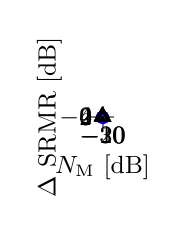
\begin{tikzpicture}[font = \small]

\begin{axis}[%
width=0.45\figurewidth,
height=0.55\figureheight,
scale only axis,
xmin=-34,
xmax=-8,
xlabel={$N_{\rm M}$ [dB]},
xlabel absolute, xlabel style={yshift=0.5em},
xmajorgrids,
ymin=-3,
ymax=6,
ylabel={$\Delta$ SRMR [dB]},
ylabel absolute, ylabel style={yshift=-1.6em},
ymajorgrids,
legend style={at=({0.005,0.005}),anchor=south west,draw=black,fill=white,legend cell align=left,row sep = -2pt}
]
\addplot [
color=blue,
dashed,
line width=1.2pt,
mark size=1.7pt,
mark=o,
mark options={solid},
]
table[row sep=crcr]{
-33 -0.181850344950451\\
-30 -0.517395573137211\\
-27 0.384383313367636\\
-24 -0.397024682435076\\
-21 0.480783567614018\\
-18 -0.63631685721368\\
-15 1.11798170226275\\
-12 -2.05719843072604\\
-9 -2.75795246963211\\
};
\addplot [
color=black,
dashed,
line width=1.0pt,
mark size=2.5pt,
mark=triangle,
mark options={solid},
]
table[row sep=crcr]{
-33 5.35139747786209\\
-30 5.31320702754899\\
-27 5.41467597144835\\
-24 5.1604741832141\\
-21 5.28289856769956\\
-18 4.45939236228628\\
-15 5.40507513902725\\
-12 3.26580823612649\\
-9 1.98060078152327\\
};
\end{axis}
\end{tikzpicture}%

                \hspace{2.1cm} (a)
        \end{subfigure}%        
        \hspace{-0.7cm}
        \begin{subfigure}[b]{0.25\textwidth}
          % This file was created by matlab2tikz v0.4.0.
% Copyright (c) 2008--2013, Nico Schlömer <nico.schloemer@gmail.com>
% All rights reserved.
% 
% The latest updates can be retrieved from
%   http://www.mathworks.com/matlabcentral/fileexchange/22022-matlab2tikz
% where you can also make suggestions and rate matlab2tikz.
% 
% 
% 

% defining custom colors
\definecolor{mycolor1}{rgb}{0,0.75,0.75}%

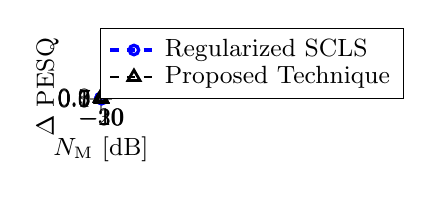
\begin{tikzpicture}[font = \small]

\begin{axis}[%
width=0.45\figurewidth,
height=0.55\figureheight,
scale only axis,
xmin=-34,
xmax=-8,
xlabel={$N_{\rm M}$ [dB]},
xlabel absolute, xlabel style={yshift=0.5em},
xmajorgrids,
ymin=0,
ymax=0.93,
ylabel={$\Delta$ PESQ},
ylabel absolute, ylabel style={yshift=-1.6em, xshift=0.4em},
ytick = {0, 0.1, 0.3, 0.5, 0.7, 0.9},
ymajorgrids,
legend style={at=({-0.48,0}),anchor=south west,draw=black,fill=white,legend cell align=left,row sep = -2pt}
]
\addplot [
color=blue,
dashed,
line width=1.2pt,
mark size=1.7pt,
mark=o,
mark options={solid}
]
table[row sep=crcr]{
-33 0.787494433408762\\
-30 0.729817481755447\\
-27 0.760350312117049\\
-24 0.753938013612263\\
-21 0.742204268442245\\
-18 0.571015525892078\\
-15 0.641969989397881\\
-12 0.214862018757196\\
-9 0.107563733409486\\
};
\addlegendentry{Regularized SCLS};

%\addplot [
%color=green!50!black,
%dashed,
%line width=1.0pt,
%mark size=2.2pt,
%mark=star,
%mark options={solid}
%]
%table[row sep=crcr]{
%-33 0.778685843810708\\
%-30 0.778952827307612\\
%-27 0.710061979452564\\
%-24 0.502397195101204\\
%-21 0.640166886768423\\
%-18 0.0094655629837801\\
%-15 0.385061962210443\\
%-12 0.0456976815362813\\
%-9 0.031725584934355\\
%};
%\addlegendentry{$G(k)$};

%\addplot [
%color=red,
%dashed,
%line width=1.2pt,
%mark size=1.8pt,
%mark=square,
%mark options={solid}
%]
%table[row sep=crcr]{
%-33 0.699169963777934\\
%-30 0.675229830027618\\
%-27 0.688247866611805\\
%-24 0.618999241873652\\
%-21 0.620255300206637\\
%-18 0.477851022832803\\
%-15 0.562020649353189\\
%-12 0.267892208848723\\
%-9 0.152526668977201\\
%};
%\addlegendntry{$G_{\delta}(k)$};

\addplot [
color=black,
dashed,
line width=1.0pt,
mark size=2.5pt,
mark=triangle,
mark options={solid}
]
table[row sep=crcr]{
-33 0.900543715497689\\
-30 0.886691062798044\\
-27 0.88030315824927\\
-24 0.79722147868595\\
-21 0.826029694942047\\
-18 0.669465711455573\\
-15 0.743701795206534\\
-12 0.36044942278444\\
-9 0.210461137082714\\
};
\addlegendentry{Proposed Technique};

\end{axis}
\end{tikzpicture}%
          
%          \vspace{-0.1cm}
          \hspace{2.4cm} (b)
        \end{subfigure}
        
        \vspace{-0.18cm}
        \caption{Performance of the regularized SCLS technique and of the proposed technique for different $N_{\rm M}$ in terms of (a) SRMR improvement and (b) PESQ score improvement.}
        \vspace{-0.3cm}
        \label{fig: srmr}
\end{figure}
The presented results show that the proposed technique yields an SRMR improvement of approximately $5.5$~dB for moderate mismatch values, whereas for high mismatch values such as $N_{\rm M} = -9$~dB the SRMR improvement is approximately $2$~dB.
On the other hand, the regularized SCLS technique often leads to a deterioration of the SRMR when compared to the unprocessed microphone signal, as indicated by the negative SRMR improvement values.
In order to compare the perceptual speech quality, Fig.~\ref{fig: srmr}(b) depicts the PESQ score improvement for both techniques.
It can be noticed that for all $N_{\rm M}$, the proposed technique yields a higher perceptual speech quality than regularized SCLS. 
As expected, the higher amount of dereverberation achieved by the proposed technique leads to a higher perceptual speech quality.

As an indication of the computational complexity of the techniques, we also state the processing time of their MATLAB implementation, including the filter design and all the necessary processing steps to obtain a final time-domain output signal.
To process a $4$~s long input signal, the proposed technique requires only $0.5$~s, whereas regularized SCLS requires approximately $4 \times 10^3$~s.

The presented experimental results illustrate that the proposed technique is not only significantly faster than SCLS, but it also results in a higher dereverberation performance and perceptual speech quality.

\section{Conclusion}
In this paper, it has been theoretically illustrated that the direct inversion of the acoustic transfer function in the frequency-domain yields undesirable tones and pre-echoes due to instability and acausality.
A novel frequency-domain inverse filtering technique has been proposed, which incorporates regularization to reduce the tones and exploits a speech enhancement scheme to reduce the pre-echoes.
Experimental results demonstrate that the proposed technique yields a higher performance and is significantly faster than the alternative SCLS inverse filtering technique.

\bibliographystyle{IEEEbib}
\bibliography{strings,refs}

\end{document}
